\documentclass[10pt,twocolumn]{article}

\usepackage[margin=0.55in]{geometry}
\usepackage{amsmath,amssymb}
\usepackage{booktabs}
\usepackage{graphicx}
\usepackage[hidelinks]{hyperref}
\usepackage{caption}
\usepackage{titlesec}
\usepackage{balance}

\titleformat{\section}{\large\bfseries}{\thesection}{0.5em}{}
\titlespacing*{\section}{0pt}{0.45em}{0.18em}
\captionsetup{font=footnotesize,labelfont=bf}
\setlength{\parindent}{0pt}
\setlength{\parskip}{0.22em}
\setlength{\columnsep}{0.23in}
\setlength{\abovedisplayskip}{0.25em}
\setlength{\belowdisplayskip}{0.25em}

\title{\vspace{-1.25em}When Usage Is a Symptom:\\ Token Billing, Quality, and Real Usage Inflation}
\author{Mini research note}
\date{\vspace{-1.0em}June 2026}

\begin{document}
\twocolumn[
\begin{@twocolumnfalse}
\maketitle
\vspace{-1.8em}

\begin{abstract}
\noindent Usage-based pricing is natural for AI products, but tokens are not ordinary units of consumption. They are an intermediate input into task completion, and their quantity is partly determined by provider choices over model quality, routing, verbosity, and retry efficiency. A simple model shows that per-token billing creates a short-run incentive to underprovide quality when lower quality increases real billable usage, while churn and reputation provide countervailing discipline. As a proof of concept, I use public Chatbot Arena preference data to compare two answers to the same prompt. The exercise does not identify intentional degradation; it shows that quality and billable usage need not be aligned. With Stripe-style metering and billing data, the same framework could distinguish valuable usage growth from avoidable friction by linking tokens, invoices, overages, downgrades, disputes, and churn.
\end{abstract}
\vspace{-0.8em}
\end{@twocolumnfalse}
]
\small

\section*{Motivation}
This note is not about fake token counts, dishonest meters, tokenizer manipulation, or cryptographic auditing. Those questions ask whether a provider over-reports usage conditional on a realized answer. The product-economics question here is different: even with honest metering, real token usage is endogenous to product quality. A weak answer can generate more billable usage through verbosity, clarification loops, hallucination correction, retries, failed tool calls, and longer conversations.

Tokens are therefore a noisy economic object. Some token growth is ``good usage'': more valuable tasks completed, deeper adoption, and higher willingness to pay. Other token growth is ``bad usage'': more friction per completed task. Under pure per-token billing, these two objects can look similar in raw revenue data even though they have opposite welfare interpretations.

\section*{A Minimal Incentive Model}
Let provider quality or efficiency be \(q\). Higher \(q\) means better task completion, fewer hallucinations, better routing, fewer retries, and less unnecessary verbosity. Expected real output token use per task is
\[
T(q),\quad T'(q)<0,
\qquad
s(q),\quad s'(q)>0.
\]
The customer pays \(B(q)=F+pT(q)\), where \(F\) is a fixed fee and \(p\) is the per-token price. Provider cost is \(C(q)=c(q)T(q)\), where \(c(q)\) may rise with model quality, stronger routing, or more expensive inference. One-period provider profit is \(\pi(q)=F+[p-c(q)]T(q)\). Holding retention fixed,
\[
\pi'(q)=-c'(q)T(q)+[p-c(q)]T'(q).
\]
Because \(T'(q)<0\), a positive token markup \(p-c(q)\) makes quality improvements reduce billable usage. If higher quality also raises unit cost, the short-run private return to quality can be below the customer return.

Retention disciplines this incentive. With customer utility \(U(q)\) increasing in success and decreasing in wasted usage, the provider solves
\[
\max_q\; F+[p-c(q)]T(q)+\beta R(U(q))\Pi,
\]
where \(R'(U)>0\). Quality degradation or inefficient routing should be more tempting when token markups are high, switching costs are high, quality is hard to diagnose, billing is delayed or opaque, reputational discipline is weak, and contracts are close to pure per-token pricing.

\section*{Proof of Concept: Chatbot Arena}
I use the public `\texttt{lmarena-ai/arena-human-preference-55k}' dataset on Hugging Face, associated with Chatbot Arena (Chiang et al., 2024). Each row is a matched task: two models answer the same prompt, and the user chooses model A, model B, or a tie. The release exposes \(57{,}477\) rows with model A/B, prompt, response A/B, and three winner indicators; it does not separately expose a both-bad label. I parse the JSON conversation strings, count visible prompt and response tokens with one common \texttt{cl100k\_base} tokenizer, and drop rows with empty prompts or responses.

For each non-tie battle \(b\), define winning and losing output tokens \(T^w_b\) and \(T^\ell_b\). The main statistic is the adverse-billing indicator
\[
A_b=\mathbf{1}\{T^\ell_b>T^w_b\}.
\]
This asks whether, within the same prompt, the lower-preferred answer would have generated more billable output usage under a pure per-token contract.

\begin{table}[!t]
\centering
\caption{Matched-response evidence from Chatbot Arena}
\vspace{-0.5em}
\resizebox{\columnwidth}{!}{\begin{tabular}{l r}
\toprule
Statistic & Estimate \\
\midrule
Non-tie Arena battles & 39,687 \\
$\Pr(T^\ell>T^w)$ & 37.7\% \\
Mean $T^\ell-T^w$ & -55 \\
Median $T^\ell-T^w$ & -34 \\
Median $T^\ell/T^w$ & 0.83 \\
90th pct. $T^\ell/T^w$ & 2.28 \\
Tie battles & 17,744 \\
Mean absolute token gap in ties & 114 \\
LPM $\beta$: $\log T^A-\log T^B$ & 0.087 (0.003) \\
Prompt controls and model FE & Yes \\
Short-prompt $\Pr(T^\ell>T^w)$ & 35.9\% \\
Long-prompt $\Pr(T^\ell>T^w)$ & 39.6\% \\
\bottomrule
\end{tabular}
}
\vspace{-0.55em}
\caption*{\scriptsize Notes: Non-tie sample excludes ties and empty prompts/responses. Tokens are visible output tokens under one common tokenizer. The LPM includes log prompt length and model A/B fixed effects; standard errors are clustered by exact prompt when prompts repeat.}
\end{table}

\begin{figure*}[!t]
\centering
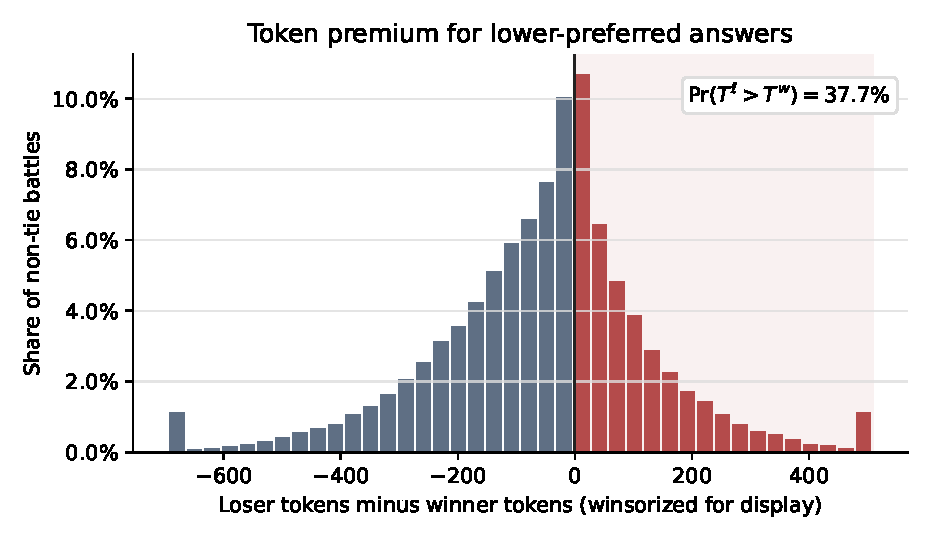
\includegraphics[width=0.66\textwidth]{../output/token_billing_quality/loser_token_premium_hist.pdf}
\vspace{-0.85em}
\caption{Distribution of loser-minus-winner output tokens. Positive values are tasks where the lower-preferred answer consumed more visible output tokens.}
\end{figure*}

\balance
\section*{Results}
Table 1 shows a mixed but useful pattern. Longer answers are rewarded on average: the fixed-effect linear probability model gives \(\hat\beta=0.087\), so a one-log-point token advantage for response A is associated with an 8.7 percentage point higher probability that A wins. This is consistent with users valuing detail in many Arena tasks.

But the wedge remains economically meaningful. In \(37.7\%\) of non-tie matched battles, the lower-preferred answer uses more output tokens than the preferred answer. The median loser is shorter than the winner, but the right tail is large: the 90th percentile of \(T^\ell/T^w\) is \(2.28\). Ties sharpen the product interpretation: in \(17{,}744\) ties, the mean absolute response-token gap is 114 tokens even though observed preference is the same. These facts do not show intent or causality. They show that billable usage and customer value are not mechanically aligned at the task level.

\section*{Mapping to Stripe Data}
Public Arena data observe prompts, answers, and preferences, but not invoices, contract terms, overages, payment events, support tickets, or churn. Stripe-style data could move from proof of concept to product measurement for AI firms that meter usage through billing events. The unit of analysis would be a customer-task or conversation episode linked to metered tokens, invoice line items, plan limits, payment failures, credits, disputes, downgrades, expansions, and retention.

The estimand is not ``tokens per customer.'' It is quality-adjusted tokens per completed task. Good usage should predict successful task completion, expansion, and retention after conditioning on customer mix and task type. Bad usage should predict retries, correction loops, support contacts, overages followed by downgrades, disputes, payment failures, or churn.

\section*{Conclusion}
Usage-based billing scales price with product intensity. For LLM products, however, usage is partly a symptom of product design and model performance. Per-token pricing can create a short-run wedge between provider revenue and user surplus because lower quality can generate more real billable usage. Retention, competition, and reputation push in the other direction. The right product metric is not tokens per customer, but quality-adjusted tokens per completed task.

\end{document}
